\documentclass[a4paper,12pt,twoside]{report}

\usepackage{acronym}
\usepackage{url}
\usepackage{cite}
\usepackage{listings}
\usepackage[pdftex]{graphicx}
\usepackage[hang,small,bf]{caption}
\usepackage{styles/tum}
\usepackage{setspace}
\usepackage[german,english]{babel}
\usepackage{float}
\usepackage{floatflt}
\usepackage{fancyhdr}
\usepackage{color}
\usepackage{booktabs}
\usepackage[pdftex,bookmarks=true,plainpages=false,pdfpagelabels=true]{hyperref}
\usepackage{mdwlist}
\usepackage{enumerate}
\usepackage{paralist}
\usepackage{array}
\usepackage{longtable}
\usepackage{listings}
\usepackage[utf8]{inputenc}
\usepackage[capitalize, noabbrev]{cleveref}

% Path for graphics
\graphicspath{{figures/}}

\begin{document}
\setlength{\evensidemargin}{22pt}
\setlength{\oddsidemargin}{22pt}

\def\doctype{Bachelor's Thesis}
\def\faculty{Informatics}
\def\title{Simulation-Based Analysis of Blockchain Architectures}		
\def\titleGer{Simulationsbasierte Analyse von Blockchain Architekturen}
\def\supervisor{Broy, Manfred; Prof. Dr. rer. nat. habil.}
\def\advisor{Marmsoler, Diego; M.Sc.}
\def\author{Leo Eichhorn}
\def\date{15.07.2018}


\hypersetup{pdfborder={0 0 0},
                        pdfauthor={<author>},
                        pdftitle={<title english>},
                        }

\lstset{showspaces=false, numbers=left, frame=single, basicstyle=\small}

\pagenumbering{alph}

\thispagestyle{empty}

\vspace{4cm}
\begin{center}
\oTUM{4cm}\\ 
\vspace{5mm}     
\huge DEPARTMENT OF INFORMATICS\\ 
\vspace{0.5cm}
\large TECHNICAL UNIVERSITY OF MUNICH\\
\vspace{1mm}
\end{center}

\vspace{13mm}

\begin{center}
{\Large \doctype\ in \faculty}
\vspace{20mm}

\begin{spacing}{1.5}
{\huge\bf \title}\\%[3ex]
\end{spacing}

\vspace{15mm}
{\LARGE \author}

\vspace{10mm}

\begin{figure}[h!]
\centering
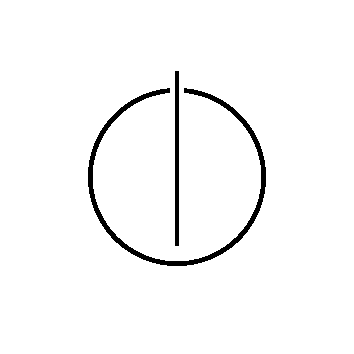
\includegraphics[width=4cm]{InformaticsLogo}
\end{figure}

\end{center}

\thispagestyle{empty}
\pagenumbering{roman}
\vspace{8mm}
\begin{center}
\oTUM{4cm}

\vspace{5mm}     
\huge DEPARTMENT OF INFORMATICS\\ 
\vspace{0.5cm}
\large TECHNICAL UNIVERSITY OF MUNICH\\
\end{center}

\vspace{5mm}

\begin{center}
{\Large \doctype\ in \faculty}
\vspace{8mm}

\begin{spacing}{1.3}
{\LARGE \title}\\
\vspace{8mm}

{\LARGE \titleGer}\\
\vspace{8mm}
\end{spacing}

\begin{tabular}{ll}
\Large Author:     & \Large \author     \\[2mm]
\Large Supervisor: & \Large \supervisor \\[2mm]				
\Large Advisor:	   & \Large \advisor    \\[2mm]
\Large Submission date:       & \Large \date
\end{tabular}

\vspace{1mm}

\begin{figure}[hb!]
\centering
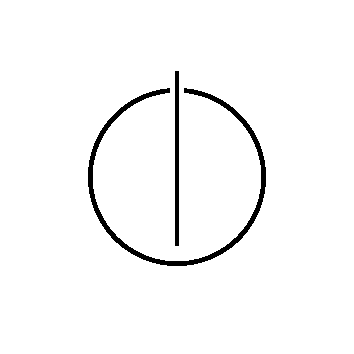
\includegraphics[width=4cm]{InformaticsLogo}
\end{figure}

\end{center}
\newpage
\thispagestyle{empty}
\mbox{}
\clearpage
\thispagestyle{empty}
\vspace*{0.8\textheight}
\noindent
I assure the single handed composition of this bachelor thesis only supported by declared resources,

\vspace{15mm}
\noindent
Munich, \date \hspace{\stretch{1}} \author
\newpage



\newpage
\thispagestyle{empty}
\mbox{}

\chapter*{Acknowledgements}


\pagenumbering{roman}

\selectlanguage{english}
\begin{abstract}

%abstract english

\textit{}

\end{abstract}

\clearpage

\selectlanguage{german}
\begin{abstract}

%abstract german
\textit{}

\end{abstract}

\clearpage

\selectlanguage{english}


\tableofcontents
\clearpage

\clearpage

\begin{acronym}
\acro{RADS}{Resistance of a blockchain architecture against double spend attacks}

\end{acronym}

\pagenumbering{arabic}

\fancyhead{}
\pagestyle{fancy}
\fancyhead[LE]{\slshape \leftmark}
\fancyhead[RO]{\slshape \rightmark}
\headheight=15pt




%------- chapter 1 -------

\chapter{Introduction}


%------- chapter 2 -------

\chapter{Background}


%------- chapter 3 -------

\chapter{Related Work}


%------- chapter 4 -------

\chapter{System design}

\section{Requirements}

\section{Overview}

\section{Design Goals}

\section{Subsystem Decomposition}


%------- chapter 5 -------

\chapter{Evaluation}

\section{Design}

\section{Objectives}

\section{Results}

\section{Findings}

\section{Discussion}

\section{Limitations}


%------- chapter 6 -------

\chapter{Model}


%------- chapter 7 -------

\chapter{Summary}

\section{Status}

\subsection{Realized Goals}

\subsection{Open Goals}

\section{Conclusion}

\section{Future Work}


\appendix

\chapter{Source Code}


\clearpage

\listoffigures
\clearpage

\listoftables
\clearpage

\bibliography{thesis}
\bibliographystyle{alpha}

\end{document}
